\section{Redes neuronales y la toma de decisiones}
\subsection{El Modelo Biol\'{o}gico}
 
 		El sistema de procesamiento de informaci\'{o}n completo est\'{a} formado en parte el
 	sistema nervioso central cuyo elemento principal es el cerebro. \'{e}ste a su vez
 	se encuentra compuesto por una unidad fundamental llamada \textit{neurona}.
 	[9] La figura \ref{fig:neuronaBio} muestra las partes de la neurona. En esta
 	se puede observar la estructura t\'{i}pica de una neurona biol\'{o}gica, la
 	cual se encuentra formada por un cuerpo celular con su n\'{u}cleo o
 	\textit{soma}, del cual se desprende, en la parte superior, una serie de
 	ramificaciones denominadas \textit{dendritas}, mientras que en la parte
 	inferior se puede observar el \textit{ax\'{o}n}, \'{e}ste es una extensi\'{o}n del soma de forma tubular y
 	tiende a ramificarse en uno de sus extremos.
 	
 	\begin{figure}[htp]
 		\centering
 		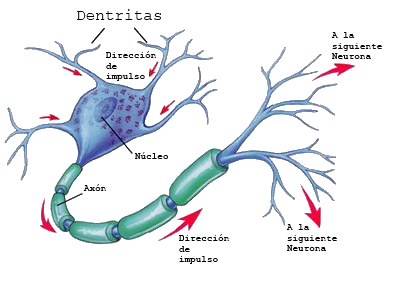
\includegraphics[width=0.5\textwidth]{images/TesisYGR-neuron.png}
 		\caption{Neurona Biol\'{o}gica}
 		\label{fig:neuronaBio}
 	\end{figure}
 	
 	 		Las neuronas son como cualquier otro tipo de c\'{e}lula, con la diferencia que
 	\'{e}stas pueden comunicarse entre s\'{i} [18]. Por lo anterior, las dendritas
 	funcionan como una canal de entrada para recibir las se�ales que provienen del
 	exterior. Estas se�ales se transfieren a una neurona por medio de una conexi\'{o}n o contacto denominado sinapsis, mientras que el ax\'{o}n transfiere los pulsos hacia otras neuronas.\\

		Las se�ales entre las neuronas pueden ser de tipo el\'{e}ctrica o sinapsis
	el\'{e}ctrica que se da cuando la sinapsis recibe una se�al el\'{e}ctrica proveniente
	de una neurona transmisora o neurona pre sin\'{a}ptica y este es transmitido al
	n\'{u}cleo de la neurona receptora o pos sin\'{a}ptica. Por otro lado la sinapsis qu\'{i}mica se distingue por no presentarse un contacto el\'{e}ctrico entre ambas partes ya que este se interrumpe por causa de un abismo o grita sin\'{a}ptico que separa un lado del otro. No obstante la informaci\'{o}n siempre fluye debido a que la se�al el\'{e}ctrica en el lado pre sin\'{a}ptico de la grita se convierte en una se�al qu\'{i}mica que atraviesa la grieta y luego se vuelve a convertir en el la receptor [9].\\
 	
 		Una caracter\'{i}stica adicional de la sinapsis es la intensidad con la que se
 	transmiten las se�ales ya que estas tienden a variar, siendo unas transferidas
 	con fuerte estimulaci\'{o}n mientras que otras de forma d\'{e}bil. Este ajuste varia
 	permitiendo que la estructura del cerebro no se mantenga fija formando conexiones m\'{a}s fuertes o d\'{e}biles seg\'{u}n se requieran ajustes.\\

 		Usando un punto de vista funcional, una neurona de forma aislada, se
 	constituye en un procesador b\'{a}sico de informaci\'{o}n que cuenta con secci\'{o}n para
 	entradas (dendritas), un \'{a}rea de procesamiento (n\'{u}cleo o soma) y secci\'{o}n de
 	salida. Con forme se aumenta el panorama se y se incluyen m\'{a}s neuronas y las interconexiones entre estas, se obtiene una red de neuronas que usan la sinapsis para poder transmitir se�ales unas a otras.
 		
 \subsection{Sistemas Expersot vs Redes Neuronales}
 
 		Como alternativa para la toma de decisiones se encuentran los sistemas
 	expertos, estos se caracterizan por contar con una base de conocimiento que
 	se encuentra separada del sistema original, permitiendo agregar nuevo
 	conocimiento a este sin requerirse realizar cambios al sistema. No obstante, se necesita una persona experta en un \'{a}rea para que se puedan crear las reglas que codifiquen el conocimiento [22].\\
 	
 		Basogain en su escrito resalta las ventajas de las redes neuronales sobre
 	estos sistemas al resaltar que el desarrollo de una red neuronal no se
 	requiere programar ni el conocimiento ni las reglas para procesar ese
 	conocimiento, ya que la es ella misma la que aprende las reglas mediante los ajustes que se realicen a las conexiones entre las neuronas.\\
 		
 		Un sistema experto hace expl\'{i}cito su conocimiento en forma de reglas pre
 	establecidas, mientras que las redes neuronales generan sus reglas
 	aprendiendo, usando como materia prima los ejemplos que le fuesen mostrados
 	durante la fase de entrenamiento de la red.\\
 		
 			La forma en que los sistemas expertos almacenan la informaci\'{o}n se ve opacada
 	por el modo empleado en las redes neuronales, ya que estas guardan su
 	conocimiento de forma distribuida a lo largo de la red y no en una sola base
 	centralizada. La caracter\'{i}stica anterior resulta una gran ventaja debido a que se pueden usar de forma asociativa, es decir, si s\'{o}lo reciben una entrada parcial la red determinar\'{a} la entrada m\'{a}s parecida en memoria y dar\'{a} una salida asociada con la entrada original completa, concedi\'{e}ndoles la capacidad de generalizar, mientras que un sistema experto requiere de la entrada completa para poder determinar la soluci\'{o}n de acuerdo a su base de conocimiento.\\

 		Finalmente, se encuentra la tolerancia a fallos, el cual se refiere al caso
 	de que si fallan partes de las neuronas simplemente se realizar\'{a}n
 	modificaciones a las conexi\'{o}n, variando \'{u}nicamente su comportamiento pero el
 	sistema en cuesti\'{o}n no deja de funcionar.
 		
 		
